\documentclass[1p]{elsarticle_modified}
%\bibliographystyle{elsarticle-num}

%\usepackage[colorlinks]{hyperref}
%\usepackage{abbrmath_seonhwa} %\Abb, \Ascr, \Acal ,\Abf, \Afrak
\usepackage{amsfonts}
\usepackage{amssymb}
\usepackage{amsmath}
\usepackage{amsthm}
\usepackage{scalefnt}
\usepackage{amsbsy}
\usepackage{kotex}
\usepackage{caption}
\usepackage{subfig}
\usepackage{color}
\usepackage{graphicx}
\usepackage{xcolor} %% white, black, red, green, blue, cyan, magenta, yellow
\usepackage{float}
\usepackage{setspace}
\usepackage{hyperref}

\usepackage{tikz}
\usetikzlibrary{arrows}

\usepackage{multirow}
\usepackage{array} % fixed length table
\usepackage{hhline}

%%%%%%%%%%%%%%%%%%%%%
\makeatletter
\renewcommand*\env@matrix[1][\arraystretch]{%
	\edef\arraystretch{#1}%
	\hskip -\arraycolsep
	\let\@ifnextchar\new@ifnextchar
	\array{*\c@MaxMatrixCols c}}
\makeatother %https://tex.stackexchange.com/questions/14071/how-can-i-increase-the-line-spacing-in-a-matrix
%%%%%%%%%%%%%%%

\usepackage[normalem]{ulem}

\newcommand{\msout}[1]{\ifmmode\text{\sout{\ensuremath{#1}}}\else\sout{#1}\fi}
%SOURCE: \msout is \stkout macro in https://tex.stackexchange.com/questions/20609/strikeout-in-math-mode

\newcommand{\cancel}[1]{
	\ifmmode
	{\color{red}\msout{#1}}
	\else
	{\color{red}\sout{#1}}
	\fi
}

\newcommand{\add}[1]{
	{\color{blue}\uwave{#1}}
}

\newcommand{\replace}[2]{
	\ifmmode
	{\color{red}\msout{#1}}{\color{blue}\uwave{#2}}
	\else
	{\color{red}\sout{#1}}{\color{blue}\uwave{#2}}
	\fi
}

\newcommand{\Sol}{\mathcal{S}} %segment
\newcommand{\D}{D} %diagram
\newcommand{\A}{\mathcal{A}} %arc


%%%%%%%%%%%%%%%%%%%%%%%%%%%%%5 test

\def\sl{\operatorname{\textup{SL}}(2,\Cbb)}
\def\psl{\operatorname{\textup{PSL}}(2,\Cbb)}
\def\quan{\mkern 1mu \triangleright \mkern 1mu}

\theoremstyle{definition}
\newtheorem{thm}{Theorem}[section]
\newtheorem{prop}[thm]{Proposition}
\newtheorem{lem}[thm]{Lemma}
\newtheorem{ques}[thm]{Question}
\newtheorem{cor}[thm]{Corollary}
\newtheorem{defn}[thm]{Definition}
\newtheorem{exam}[thm]{Example}
\newtheorem{rmk}[thm]{Remark}
\newtheorem{alg}[thm]{Algorithm}

\newcommand{\I}{\sqrt{-1}}
\begin{document}

%\begin{frontmatter}
%
%\title{Boundary parabolic representations of knots up to 8 crossings}
%
%%% Group authors per affiliation:
%\author{Yunhi Cho} 
%\address{Department of Mathematics, University of Seoul, Seoul, Korea}
%\ead{yhcho@uos.ac.kr}
%
%
%\author{Seonhwa Kim} %\fnref{s_kim}}
%\address{Center for Geometry and Physics, Institute for Basic Science, Pohang, 37673, Korea}
%\ead{ryeona17@ibs.re.kr}
%
%\author{Hyuk Kim}
%\address{Department of Mathematical Sciences, Seoul National University, Seoul 08826, Korea}
%\ead{hyukkim@snu.ac.kr}
%
%\author{Seokbeom Yoon}
%\address{Department of Mathematical Sciences, Seoul National University, Seoul, 08826,  Korea}
%\ead{sbyoon15@snu.ac.kr}
%
%\begin{abstract}
%We find all boundary parabolic representation of knots up to 8 crossings.
%
%\end{abstract}
%\begin{keyword}
%    \MSC[2010] 57M25 
%\end{keyword}
%
%\end{frontmatter}

%\linenumbers
%\tableofcontents
%
\newcommand\colored[1]{\textcolor{white}{\rule[-0.35ex]{0.8em}{1.4ex}}\kern-0.8em\color{red} #1}%
%\newcommand\colored[1]{\textcolor{white}{ #1}\kern-2.17ex	\textcolor{white}{ #1}\kern-1.81ex	\textcolor{white}{ #1}\kern-2.15ex\color{red}#1	}

{\Large $\underline{9_{30}~(K9a_{1})}$}

\setlength{\tabcolsep}{10pt}
\renewcommand{\arraystretch}{1.6}
\vspace{1cm}\begin{tabular}{m{100pt}>{\centering\arraybackslash}m{274pt}}
\multirow{5}{120pt}{
	\centering
	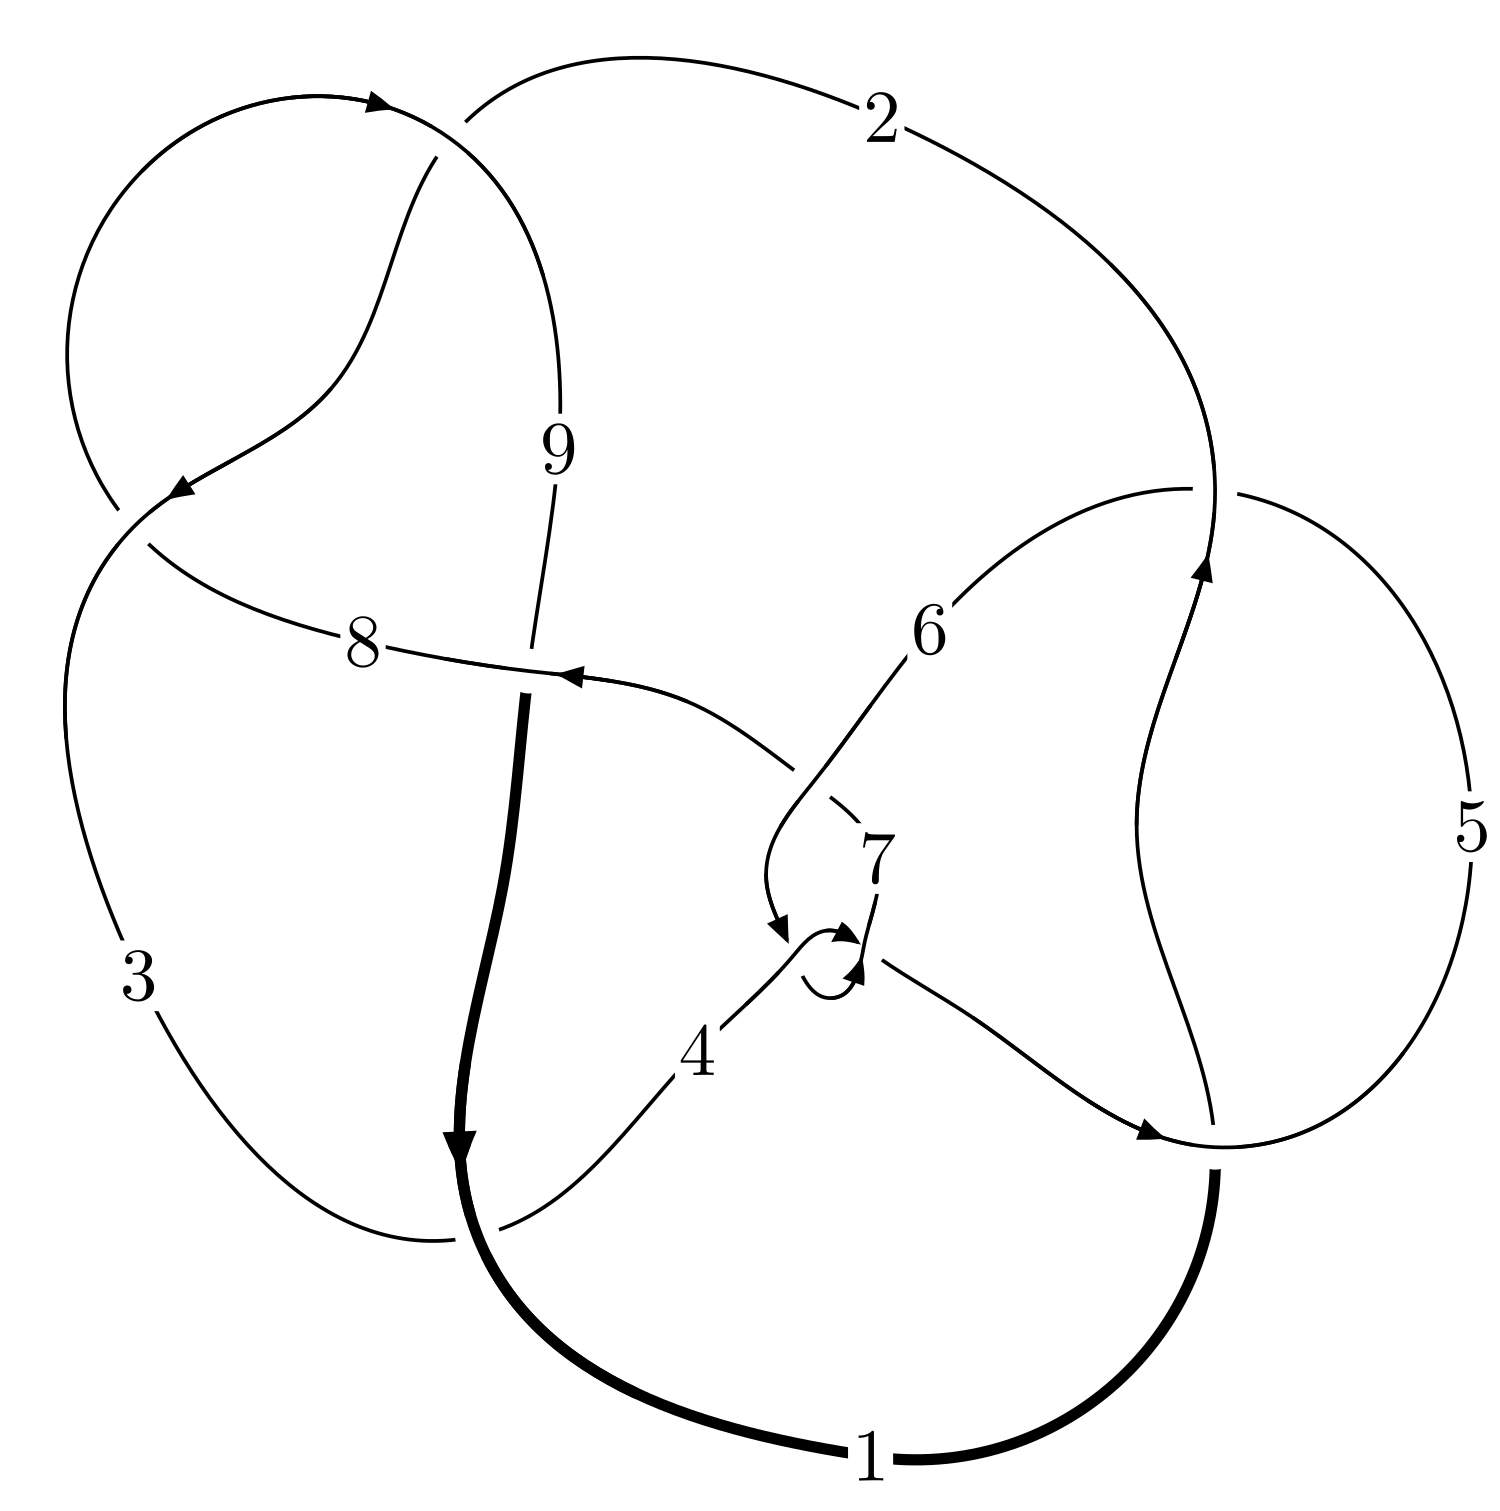
\includegraphics[width=112pt]{../../../GIT/diagram.site/Diagrams/png/65_9_30.png}\\
\ \ \ A knot diagram\footnotemark}&
\allowdisplaybreaks
\textbf{Linearized knot diagam} \\
\cline{2-2}
 &
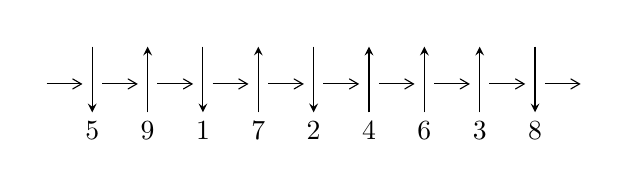
\begin{tikzpicture}[x=20pt, y=17pt]
	% nodes
	\node (C0) at (0, 0) {};
	\node (C1) at (1, 0) {};
	\node (C1U) at (1, +1) {};
	\node (C1D) at (1, -1) {5};

	\node (C2) at (2, 0) {};
	\node (C2U) at (2, +1) {};
	\node (C2D) at (2, -1) {9};

	\node (C3) at (3, 0) {};
	\node (C3U) at (3, +1) {};
	\node (C3D) at (3, -1) {1};

	\node (C4) at (4, 0) {};
	\node (C4U) at (4, +1) {};
	\node (C4D) at (4, -1) {7};

	\node (C5) at (5, 0) {};
	\node (C5U) at (5, +1) {};
	\node (C5D) at (5, -1) {2};

	\node (C6) at (6, 0) {};
	\node (C6U) at (6, +1) {};
	\node (C6D) at (6, -1) {4};

	\node (C7) at (7, 0) {};
	\node (C7U) at (7, +1) {};
	\node (C7D) at (7, -1) {6};

	\node (C8) at (8, 0) {};
	\node (C8U) at (8, +1) {};
	\node (C8D) at (8, -1) {3};

	\node (C9) at (9, 0) {};
	\node (C9U) at (9, +1) {};
	\node (C9D) at (9, -1) {8};
	\node (C10) at (10, 0) {};

	% arrows
	\draw[->,>={angle 60}]
	(C0) edge (C1) (C1) edge (C2) (C2) edge (C3) (C3) edge (C4) (C4) edge (C5) (C5) edge (C6) (C6) edge (C7) (C7) edge (C8) (C8) edge (C9) (C9) edge (C10) ;	\draw[->,>=stealth]
	(C1U) edge (C1D) (C2D) edge (C2U) (C3U) edge (C3D) (C4D) edge (C4U) (C5U) edge (C5D) (C6D) edge (C6U) (C7D) edge (C7U) (C8D) edge (C8U) (C9U) edge (C9D) ;
	\end{tikzpicture} \\
\hhline{~~} \\& 
\textbf{Solving Sequence} \\ \cline{2-2} 
 &
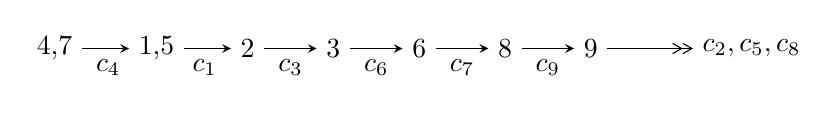
\begin{tikzpicture}[x=31pt, y=7pt]
	% node
	\node (A0) at (-1/8, 0) {4,7};
	\node (A1) at (17/16, 0) {1,5};
	\node (A2) at (17/8, 0) {2};
	\node (A3) at (25/8, 0) {3};
	\node (A4) at (33/8, 0) {6};
	\node (A5) at (41/8, 0) {8};
	\node (A6) at (49/8, 0) {9};
	\node (C1) at (1/2, -1) {$c_{4}$};
	\node (C2) at (13/8, -1) {$c_{1}$};
	\node (C3) at (21/8, -1) {$c_{3}$};
	\node (C4) at (29/8, -1) {$c_{6}$};
	\node (C5) at (37/8, -1) {$c_{7}$};
	\node (C6) at (45/8, -1) {$c_{9}$};
	\node (A7) at (8, 0) {$c_{2},c_{5},c_{8}$};

	% edge
	\draw[->,>=stealth]	
	(A0) edge (A1) (A1) edge (A2) (A2) edge (A3) (A3) edge (A4) (A4) edge (A5) (A5) edge (A6) ;
	\draw[->>,>={angle 60}]	
	(A6) edge (A7);
\end{tikzpicture} \\ 

\end{tabular} \\

\footnotetext{
The image of knot diagram is generated by the software ``\textbf{Draw programme}" developed by Andrew Bartholomew(\url{http://www.layer8.co.uk/maths/draw/index.htm\#Running-draw}), where we modified some parts for our purpose(\url{https://github.com/CATsTAILs/LinksPainter}).
}\phantom \\ \newline 
\centering \textbf{Ideals for irreducible components\footnotemark of $X_{\text{par}}$} 
 
\begin{align*}
I^u_{1}&=\langle 
u^{27}-4 u^{26}+\cdots+2 b-3,\;-5 u^{27}+14 u^{26}+\cdots+2 a+9,\;u^{28}-3 u^{27}+\cdots- u+1\rangle \\
I^u_{2}&=\langle 
b+a,\;a^2- a+1,\;u+1\rangle \\
\\
\end{align*}
\raggedright * 2 irreducible components of $\dim_{\mathbb{C}}=0$, with total 30 representations.\\
\footnotetext{All coefficients of polynomials are rational numbers. But the coefficients are sometimes approximated in decimal forms when there is not enough margin.}
\newpage
\renewcommand{\arraystretch}{1}
\centering \section*{I. $I^u_{1}= \langle u^{27}-4 u^{26}+\cdots+2 b-3,\;-5 u^{27}+14 u^{26}+\cdots+2 a+9,\;u^{28}-3 u^{27}+\cdots- u+1 \rangle$}
\flushleft \textbf{(i) Arc colorings}\\
\begin{tabular}{m{7pt} m{180pt} m{7pt} m{180pt} }
\flushright $a_{4}=$&$\begin{pmatrix}1\\0\end{pmatrix}$ \\
\flushright $a_{7}=$&$\begin{pmatrix}0\\u\end{pmatrix}$ \\
\flushright $a_{1}=$&$\begin{pmatrix}\frac{5}{2} u^{27}-7 u^{26}+\cdots+2 u-\frac{9}{2}\\-\frac{1}{2} u^{27}+2 u^{26}+\cdots+2 u+\frac{3}{2}\end{pmatrix}$ \\
\flushright $a_{5}=$&$\begin{pmatrix}1\\- u^2\end{pmatrix}$ \\
\flushright $a_{2}=$&$\begin{pmatrix}\frac{9}{2} u^{27}-10 u^{26}+\cdots+2 u-\frac{11}{2}\\-\frac{7}{2} u^{27}+9 u^{26}+\cdots+u+\frac{9}{2}\end{pmatrix}$ \\
\flushright $a_{3}=$&$\begin{pmatrix}\frac{1}{2} u^{27}- u^{26}+\cdots+u+\frac{3}{2}\\-\frac{1}{2} u^{27}+u^{26}+\cdots- u+\frac{1}{2}\end{pmatrix}$ \\
\flushright $a_{6}=$&$\begin{pmatrix}- u\\u\end{pmatrix}$ \\
\flushright $a_{8}=$&$\begin{pmatrix}u^3\\- u^3+u\end{pmatrix}$ \\
\flushright $a_{9}=$&$\begin{pmatrix}4 u^{27}-9 u^{26}+\cdots+3 u-5\\-\frac{5}{2} u^{27}+6 u^{26}+\cdots+2 u+\frac{7}{2}\end{pmatrix}$\\ \flushright $a_{9}=$&$\begin{pmatrix}4 u^{27}-9 u^{26}+\cdots+3 u-5\\-\frac{5}{2} u^{27}+6 u^{26}+\cdots+2 u+\frac{7}{2}\end{pmatrix}$\\&\end{tabular}
\flushleft \textbf{(ii) Obstruction class $= -1$}\\~\\
\flushleft \textbf{(iii) Cusp Shapes $= u^{27}- u^{26}-3 u^{25}+6 u^{24}-5 u^{22}+13 u^{21}-24 u^{20}-3 u^{19}+81 u^{18}-69 u^{17}-92 u^{16}+190 u^{15}+6 u^{14}-242 u^{13}+142 u^{12}+176 u^{11}-212 u^{10}-40 u^9+182 u^8-38 u^7-93 u^6+53 u^5+30 u^4-29 u^3- u^2+9 u$}\\~\\
\newpage\renewcommand{\arraystretch}{1}
\flushleft \textbf{(iv) u-Polynomials at the component}\newline \\
\begin{tabular}{m{50pt}|m{274pt}}
Crossings & \hspace{64pt}u-Polynomials at each crossing \\
\hline $$\begin{aligned}c_{1},c_{5}\end{aligned}$$&$\begin{aligned}
&u^{28}+u^{27}+\cdots+8 u+4
\end{aligned}$\\
\hline $$\begin{aligned}c_{2},c_{8}\end{aligned}$$&$\begin{aligned}
&u^{28}+2 u^{27}+\cdots+2 u+1
\end{aligned}$\\
\hline $$\begin{aligned}c_{3}\end{aligned}$$&$\begin{aligned}
&u^{28}-2 u^{27}+\cdots-22 u+17
\end{aligned}$\\
\hline $$\begin{aligned}c_{4},c_{6}\end{aligned}$$&$\begin{aligned}
&u^{28}+3 u^{27}+\cdots+u+1
\end{aligned}$\\
\hline $$\begin{aligned}c_{7}\end{aligned}$$&$\begin{aligned}
&u^{28}-13 u^{27}+\cdots+7 u+1
\end{aligned}$\\
\hline $$\begin{aligned}c_{9}\end{aligned}$$&$\begin{aligned}
&u^{28}+14 u^{27}+\cdots+2 u+1
\end{aligned}$\\
\hline
\end{tabular}\\~\\
\newpage\renewcommand{\arraystretch}{1}
\flushleft \textbf{(v) Riley Polynomials at the component}\newline \\
\begin{tabular}{m{50pt}|m{274pt}}
Crossings & \hspace{64pt}Riley Polynomials at each crossing \\
\hline $$\begin{aligned}c_{1},c_{5}\end{aligned}$$&$\begin{aligned}
&y^{28}-15 y^{27}+\cdots-88 y+16
\end{aligned}$\\
\hline $$\begin{aligned}c_{2},c_{8}\end{aligned}$$&$\begin{aligned}
&y^{28}+14 y^{27}+\cdots+2 y+1
\end{aligned}$\\
\hline $$\begin{aligned}c_{3}\end{aligned}$$&$\begin{aligned}
&y^{28}-10 y^{27}+\cdots-246 y+289
\end{aligned}$\\
\hline $$\begin{aligned}c_{4},c_{6}\end{aligned}$$&$\begin{aligned}
&y^{28}-13 y^{27}+\cdots+7 y+1
\end{aligned}$\\
\hline $$\begin{aligned}c_{7}\end{aligned}$$&$\begin{aligned}
&y^{28}+7 y^{27}+\cdots-61 y+1
\end{aligned}$\\
\hline $$\begin{aligned}c_{9}\end{aligned}$$&$\begin{aligned}
&y^{28}+2 y^{27}+\cdots+14 y+1
\end{aligned}$\\
\hline
\end{tabular}\\~\\
\newpage\flushleft \textbf{(vi) Complex Volumes and Cusp Shapes}
$$\begin{array}{c|c|c}  
\text{Solutions to }I^u_{1}& \I (\text{vol} + \sqrt{-1}CS) & \text{Cusp shape}\\
 \hline 
\begin{aligned}
u &= \phantom{-}0.421904 + 0.904838 I \\
a &= -0.038492 - 0.189970 I \\
b &= -1.43260 - 0.55257 I\end{aligned}
 & -5.32101 - 6.23266 I & -4.14975 + 4.30079 I \\ \hline\begin{aligned}
u &= \phantom{-}0.421904 - 0.904838 I \\
a &= -0.038492 + 0.189970 I \\
b &= -1.43260 + 0.55257 I\end{aligned}
 & -5.32101 + 6.23266 I & -4.14975 - 4.30079 I \\ \hline\begin{aligned}
u &= -0.959758 + 0.402988 I \\
a &= -0.766770 + 1.057520 I \\
b &= -0.623667 - 0.562813 I\end{aligned}
 & \phantom{-}1.85217 - 1.40144 I & \phantom{-}4.69947 + 1.74630 I \\ \hline\begin{aligned}
u &= -0.959758 - 0.402988 I \\
a &= -0.766770 - 1.057520 I \\
b &= -0.623667 + 0.562813 I\end{aligned}
 & \phantom{-}1.85217 + 1.40144 I & \phantom{-}4.69947 - 1.74630 I \\ \hline\begin{aligned}
u &= \phantom{-}0.619172 + 0.839658 I \\
a &= -0.016226 + 0.286921 I \\
b &= -1.019470 - 0.068324 I\end{aligned}
 & -6.61232 + 2.08114 I & -5.79595 - 2.78862 I \\ \hline\begin{aligned}
u &= \phantom{-}0.619172 - 0.839658 I \\
a &= -0.016226 - 0.286921 I \\
b &= -1.019470 + 0.068324 I\end{aligned}
 & -6.61232 - 2.08114 I & -5.79595 + 2.78862 I \\ \hline\begin{aligned}
u &= \phantom{-}0.963620 + 0.456689 I \\
a &= \phantom{-}0.72093 + 1.60659 I \\
b &= -0.015157 - 1.395580 I\end{aligned}
 & \phantom{-}1.56772 + 4.24816 I & \phantom{-}1.88645 - 6.97904 I \\ \hline\begin{aligned}
u &= \phantom{-}0.963620 - 0.456689 I \\
a &= \phantom{-}0.72093 - 1.60659 I \\
b &= -0.015157 + 1.395580 I\end{aligned}
 & \phantom{-}1.56772 - 4.24816 I & \phantom{-}1.88645 + 6.97904 I \\ \hline\begin{aligned}
u &= \phantom{-}0.855481 + 0.371946 I \\
a &= -1.18245 - 1.31391 I \\
b &= \phantom{-}0.66840 + 1.28739 I\end{aligned}
 & \phantom{-}0.967687 - 0.906276 I & -0.59768 - 1.67094 I \\ \hline\begin{aligned}
u &= \phantom{-}0.855481 - 0.371946 I \\
a &= -1.18245 + 1.31391 I \\
b &= \phantom{-}0.66840 - 1.28739 I\end{aligned}
 & \phantom{-}0.967687 + 0.906276 I & -0.59768 + 1.67094 I\\
 \hline 
 \end{array}$$\newpage$$\begin{array}{c|c|c}  
\text{Solutions to }I^u_{1}& \I (\text{vol} + \sqrt{-1}CS) & \text{Cusp shape}\\
 \hline 
\begin{aligned}
u &= \phantom{-}0.454354 + 0.784849 I \\
a &= -0.204179 + 0.058390 I \\
b &= \phantom{-}1.105360 + 0.510425 I\end{aligned}
 & -2.52313 - 1.47542 I & -1.29345 + 0.59666 I \\ \hline\begin{aligned}
u &= \phantom{-}0.454354 - 0.784849 I \\
a &= -0.204179 - 0.058390 I \\
b &= \phantom{-}1.105360 - 0.510425 I\end{aligned}
 & -2.52313 + 1.47542 I & -1.29345 - 0.59666 I \\ \hline\begin{aligned}
u &= -0.962167 + 0.550809 I \\
a &= \phantom{-}0.83827 - 1.25040 I \\
b &= \phantom{-}1.191130 + 0.619206 I\end{aligned}
 & -0.41268 - 5.75423 I & \phantom{-}0.10698 + 5.96655 I \\ \hline\begin{aligned}
u &= -0.962167 - 0.550809 I \\
a &= \phantom{-}0.83827 + 1.25040 I \\
b &= \phantom{-}1.191130 - 0.619206 I\end{aligned}
 & -0.41268 + 5.75423 I & \phantom{-}0.10698 - 5.96655 I \\ \hline\begin{aligned}
u &= -1.126550 + 0.202617 I \\
a &= -0.903208 + 0.571058 I \\
b &= \phantom{-}0.236722 - 0.655524 I\end{aligned}
 & \phantom{-}2.40233 - 0.64414 I & \phantom{-}4.35398 - 1.30683 I \\ \hline\begin{aligned}
u &= -1.126550 - 0.202617 I \\
a &= -0.903208 - 0.571058 I \\
b &= \phantom{-}0.236722 + 0.655524 I\end{aligned}
 & \phantom{-}2.40233 + 0.64414 I & \phantom{-}4.35398 + 1.30683 I \\ \hline\begin{aligned}
u &= -0.668097 + 0.525777 I \\
a &= \phantom{-}0.55770 - 1.31624 I \\
b &= \phantom{-}0.847077 - 0.345927 I\end{aligned}
 & -1.32210 + 1.34593 I & -1.91932 - 0.66126 I \\ \hline\begin{aligned}
u &= -0.668097 - 0.525777 I \\
a &= \phantom{-}0.55770 + 1.31624 I \\
b &= \phantom{-}0.847077 + 0.345927 I\end{aligned}
 & -1.32210 - 1.34593 I & -1.91932 + 0.66126 I \\ \hline\begin{aligned}
u &= \phantom{-}1.021030 + 0.695890 I \\
a &= \phantom{-}0.04209 - 1.42194 I \\
b &= -0.763781 + 0.287418 I\end{aligned}
 & -5.39487 + 3.62399 I & -4.20871 - 2.76186 I \\ \hline\begin{aligned}
u &= \phantom{-}1.021030 - 0.695890 I \\
a &= \phantom{-}0.04209 + 1.42194 I \\
b &= -0.763781 - 0.287418 I\end{aligned}
 & -5.39487 - 3.62399 I & -4.20871 + 2.76186 I\\
 \hline 
 \end{array}$$\newpage$$\begin{array}{c|c|c}  
\text{Solutions to }I^u_{1}& \I (\text{vol} + \sqrt{-1}CS) & \text{Cusp shape}\\
 \hline 
\begin{aligned}
u &= \phantom{-}1.099170 + 0.618751 I \\
a &= \phantom{-}0.03996 + 1.72641 I \\
b &= \phantom{-}1.13985 - 0.88919 I\end{aligned}
 & -0.59978 + 6.77427 I & \phantom{-}1.77406 - 4.95962 I \\ \hline\begin{aligned}
u &= \phantom{-}1.099170 - 0.618751 I \\
a &= \phantom{-}0.03996 - 1.72641 I \\
b &= \phantom{-}1.13985 + 0.88919 I\end{aligned}
 & -0.59978 - 6.77427 I & \phantom{-}1.77406 + 4.95962 I \\ \hline\begin{aligned}
u &= -1.278740 + 0.117832 I \\
a &= \phantom{-}1.225830 - 0.293847 I \\
b &= -0.991759 + 0.593054 I\end{aligned}
 & \phantom{-}0.65193 + 3.28147 I & -1.23266 - 4.99392 I \\ \hline\begin{aligned}
u &= -1.278740 - 0.117832 I \\
a &= \phantom{-}1.225830 + 0.293847 I \\
b &= -0.991759 - 0.593054 I\end{aligned}
 & \phantom{-}0.65193 - 3.28147 I & -1.23266 + 4.99392 I \\ \hline\begin{aligned}
u &= \phantom{-}1.146350 + 0.652255 I \\
a &= \phantom{-}0.11235 - 1.78840 I \\
b &= -1.53314 + 0.75996 I\end{aligned}
 & -3.12706 + 11.95450 I & -1.04116 - 8.32221 I \\ \hline\begin{aligned}
u &= \phantom{-}1.146350 - 0.652255 I \\
a &= \phantom{-}0.11235 + 1.78840 I \\
b &= -1.53314 - 0.75996 I\end{aligned}
 & -3.12706 - 11.95450 I & -1.04116 + 8.32221 I \\ \hline\begin{aligned}
u &= -0.085781 + 0.348606 I \\
a &= -0.92580 + 1.34078 I \\
b &= \phantom{-}0.191038 + 0.606129 I\end{aligned}
 & -0.22315 - 1.43304 I & -1.58225 + 4.97603 I \\ \hline\begin{aligned}
u &= -0.085781 - 0.348606 I \\
a &= -0.92580 - 1.34078 I \\
b &= \phantom{-}0.191038 - 0.606129 I\end{aligned}
 & -0.22315 + 1.43304 I & -1.58225 - 4.97603 I\\
 \hline 
 \end{array}$$\newpage\newpage\renewcommand{\arraystretch}{1}
\centering \section*{II. $I^u_{2}= \langle b+a,\;a^2- a+1,\;u+1 \rangle$}
\flushleft \textbf{(i) Arc colorings}\\
\begin{tabular}{m{7pt} m{180pt} m{7pt} m{180pt} }
\flushright $a_{4}=$&$\begin{pmatrix}1\\0\end{pmatrix}$ \\
\flushright $a_{7}=$&$\begin{pmatrix}0\\-1\end{pmatrix}$ \\
\flushright $a_{1}=$&$\begin{pmatrix}a\\- a\end{pmatrix}$ \\
\flushright $a_{5}=$&$\begin{pmatrix}1\\-1\end{pmatrix}$ \\
\flushright $a_{2}=$&$\begin{pmatrix}a\\- a\end{pmatrix}$ \\
\flushright $a_{3}=$&$\begin{pmatrix}a\\- a+1\end{pmatrix}$ \\
\flushright $a_{6}=$&$\begin{pmatrix}1\\-1\end{pmatrix}$ \\
\flushright $a_{8}=$&$\begin{pmatrix}-1\\0\end{pmatrix}$ \\
\flushright $a_{9}=$&$\begin{pmatrix}0\\- a\end{pmatrix}$\\ \flushright $a_{9}=$&$\begin{pmatrix}0\\- a\end{pmatrix}$\\&\end{tabular}
\flushleft \textbf{(ii) Obstruction class $= 1$}\\~\\
\flushleft \textbf{(iii) Cusp Shapes $= 4 a+1$}\\~\\
\newpage\renewcommand{\arraystretch}{1}
\flushleft \textbf{(iv) u-Polynomials at the component}\newline \\
\begin{tabular}{m{50pt}|m{274pt}}
Crossings & \hspace{64pt}u-Polynomials at each crossing \\
\hline $$\begin{aligned}c_{1},c_{5}\end{aligned}$$&$\begin{aligned}
&u^2
\end{aligned}$\\
\hline $$\begin{aligned}c_{2}\end{aligned}$$&$\begin{aligned}
&u^2- u+1
\end{aligned}$\\
\hline $$\begin{aligned}c_{3},c_{8},c_{9}\end{aligned}$$&$\begin{aligned}
&u^2+u+1
\end{aligned}$\\
\hline $$\begin{aligned}c_{4}\end{aligned}$$&$\begin{aligned}
&(u+1)^2
\end{aligned}$\\
\hline $$\begin{aligned}c_{6},c_{7}\end{aligned}$$&$\begin{aligned}
&(u-1)^2
\end{aligned}$\\
\hline
\end{tabular}\\~\\
\newpage\renewcommand{\arraystretch}{1}
\flushleft \textbf{(v) Riley Polynomials at the component}\newline \\
\begin{tabular}{m{50pt}|m{274pt}}
Crossings & \hspace{64pt}Riley Polynomials at each crossing \\
\hline $$\begin{aligned}c_{1},c_{5}\end{aligned}$$&$\begin{aligned}
&y^2
\end{aligned}$\\
\hline $$\begin{aligned}c_{2},c_{3},c_{8}\\c_{9}\end{aligned}$$&$\begin{aligned}
&y^2+y+1
\end{aligned}$\\
\hline $$\begin{aligned}c_{4},c_{6},c_{7}\end{aligned}$$&$\begin{aligned}
&(y-1)^2
\end{aligned}$\\
\hline
\end{tabular}\\~\\
\newpage\flushleft \textbf{(vi) Complex Volumes and Cusp Shapes}
$$\begin{array}{c|c|c}  
\text{Solutions to }I^u_{2}& \I (\text{vol} + \sqrt{-1}CS) & \text{Cusp shape}\\
 \hline 
\begin{aligned}
u &= -1.00000\phantom{ +0.000000I} \\
a &= \phantom{-}0.500000 + 0.866025 I \\
b &= -0.500000 - 0.866025 I\end{aligned}
 & \phantom{-}1.64493 - 2.02988 I & \phantom{-}3.00000 + 3.46410 I \\ \hline\begin{aligned}
u &= -1.00000\phantom{ +0.000000I} \\
a &= \phantom{-}0.500000 - 0.866025 I \\
b &= -0.500000 + 0.866025 I\end{aligned}
 & \phantom{-}1.64493 + 2.02988 I & \phantom{-}3.00000 - 3.46410 I\\
 \hline 
 \end{array}$$\newpage
\newpage\renewcommand{\arraystretch}{1}
\centering \section*{ III. u-Polynomials}
\begin{tabular}{m{50pt}|m{274pt}}
Crossings & \hspace{64pt}u-Polynomials at each crossing \\
\hline $$\begin{aligned}c_{1},c_{5}\end{aligned}$$&$\begin{aligned}
&u^2(u^{28}+u^{27}+\cdots+8 u+4)
\end{aligned}$\\
\hline $$\begin{aligned}c_{2}\end{aligned}$$&$\begin{aligned}
&(u^2- u+1)(u^{28}+2 u^{27}+\cdots+2 u+1)
\end{aligned}$\\
\hline $$\begin{aligned}c_{3}\end{aligned}$$&$\begin{aligned}
&(u^2+u+1)(u^{28}-2 u^{27}+\cdots-22 u+17)
\end{aligned}$\\
\hline $$\begin{aligned}c_{4}\end{aligned}$$&$\begin{aligned}
&((u+1)^2)(u^{28}+3 u^{27}+\cdots+u+1)
\end{aligned}$\\
\hline $$\begin{aligned}c_{6}\end{aligned}$$&$\begin{aligned}
&((u-1)^2)(u^{28}+3 u^{27}+\cdots+u+1)
\end{aligned}$\\
\hline $$\begin{aligned}c_{7}\end{aligned}$$&$\begin{aligned}
&((u-1)^2)(u^{28}-13 u^{27}+\cdots+7 u+1)
\end{aligned}$\\
\hline $$\begin{aligned}c_{8}\end{aligned}$$&$\begin{aligned}
&(u^2+u+1)(u^{28}+2 u^{27}+\cdots+2 u+1)
\end{aligned}$\\
\hline $$\begin{aligned}c_{9}\end{aligned}$$&$\begin{aligned}
&(u^2+u+1)(u^{28}+14 u^{27}+\cdots+2 u+1)
\end{aligned}$\\
\hline
\end{tabular}\newpage\renewcommand{\arraystretch}{1}
\centering \section*{ IV. Riley Polynomials}
\begin{tabular}{m{50pt}|m{274pt}}
Crossings & \hspace{64pt}Riley Polynomials at each crossing \\
\hline $$\begin{aligned}c_{1},c_{5}\end{aligned}$$&$\begin{aligned}
&y^2(y^{28}-15 y^{27}+\cdots-88 y+16)
\end{aligned}$\\
\hline $$\begin{aligned}c_{2},c_{8}\end{aligned}$$&$\begin{aligned}
&(y^2+y+1)(y^{28}+14 y^{27}+\cdots+2 y+1)
\end{aligned}$\\
\hline $$\begin{aligned}c_{3}\end{aligned}$$&$\begin{aligned}
&(y^2+y+1)(y^{28}-10 y^{27}+\cdots-246 y+289)
\end{aligned}$\\
\hline $$\begin{aligned}c_{4},c_{6}\end{aligned}$$&$\begin{aligned}
&((y-1)^2)(y^{28}-13 y^{27}+\cdots+7 y+1)
\end{aligned}$\\
\hline $$\begin{aligned}c_{7}\end{aligned}$$&$\begin{aligned}
&((y-1)^2)(y^{28}+7 y^{27}+\cdots-61 y+1)
\end{aligned}$\\
\hline $$\begin{aligned}c_{9}\end{aligned}$$&$\begin{aligned}
&(y^2+y+1)(y^{28}+2 y^{27}+\cdots+14 y+1)
\end{aligned}$\\
\hline
\end{tabular}
\vskip 2pc
\end{document}